%%%%%%%%%%%%%%%%%%%%%%%%%%%%%%%%%%%%%%%%%
% University Assignment Title Page 
% LaTeX Template
% Version 1.0 (27/12/12)
%
% This template has been downloaded from:
% http://www.LaTeXTemplates.com
%
% Original author:
% WikiBooks (http://en.wikibooks.org/wiki/LaTeX/Title_Creation)
%
% License:
% CC BY-NC-SA 3.0 (http://creativecommons.org/licenses/by-nc-sa/3.0/)
% 
% Instructions for using this template:
% This title page is capable of being compiled as is. This is not useful for 
% including it in another document. To do this, you have two options: 
%
% 1) Copy/paste everything between \begin{document} and \end{document} 
% starting at \begin{titlepage} and paste this into another LaTeX file where you 
% want your title page.
% OR
% 2) Remove everything outside the \begin{titlepage} and \end{titlepage} and 
% move this file to the same directory as the LaTeX file you wish to add it to. 
% Then add \input{./title_page_1.tex} to your LaTeX file where you want your
% title page.
%
%%%%%%%%%%%%%%%%%%%%%%%%%%%%%%%%%%%%%%%%%

%----------------------------------------------------------------------------------------
%	PACKAGES AND OTHER DOCUMENT CONFIGURATIONS
%----------------------------------------------------------------------------------------

\documentclass[12pt]{article}
\usepackage{graphicx}
\begin{document}

\begin{titlepage}

\newcommand{\HRule}{\rule{\linewidth}{0.5mm}} % Defines a new command for the horizontal lines, change thickness here


 
%----------------------------------------------------------------------------------------

\center % Center everything on the page
 
%----------------------------------------------------------------------------------------
%	HEADING SECTIONS
%----------------------------------------------------------------------------------------


%----------------------------------------------------------------------------------------
%	LOGO SECTION
%----------------------------------------------------------------------------------------


\includegraphics{logo_epfl-eps-converted-to}\\[1cm] % Include a department/university logo - this will require the graphicx package

%\textsc{\LARGE \'Ecole Polytechnique F\'ed\'erale de Lausanne}\\[1.5cm] % Name of your university/college
\textsc{\Large Biological Modeling of Neural Networks}\\[0.5cm] % Major heading such as course name

%----------------------------------------------------------------------------------------
%	TITLE SECTION
%----------------------------------------------------------------------------------------

\HRule \\[0.4cm]
{ \huge \bfseries Hopfield Model}\\[0.4cm] % Title of your document

\textsc{\large Storage of Sequences of patterns in asymetric hopfield networks with delayed synapses}\\[0.5cm] % Minor heading such as course title

\HRule \\[1.5cm]

%----------------------------------------------------------------------------------------
%	AUTHOR SECTION
%----------------------------------------------------------------------------------------

\begin{flushright}
\large Miryam \textsc{Chaabouni}

\large Joseph \textsc{Lemaitre}\\ % Your name

\end{flushright}


% If you don't want a supervisor, uncomment the two lines below and remove the section above
%\Large \emph{Author:}\\
%John \textsc{Smith}\\[3cm] % Your name

%----------------------------------------------------------------------------------------
%	DATE SECTION
%----------------------------------------------------------------------------------------

%{\large \today}\\[3cm] % Date, change the \today to a set date if you want to be precise

\vfill % Fill the rest of the page with whitespace

\end{titlepage}

\section{Exercise 1 : Standard Hopfield Network }
\subsection{Exercise 1.1 : Implementation}
We created a class hopfieldNetwork which has the following attributes : 
\begin{itemize}
\item N : number of neurons 
\item pattern : array of $P\times N$ states, where P is the number of patterns 
\item weight : array of $N\times N$ that represents the matrix of interaction between neurons
\item x : state of the network at each time step, e.g.,  $x = \{1, -1, -1, \dots\}$
\end{itemize}
and the following functions : 
\begin{description}
\item [\_\_init\_\_] creates an instance of the class hofieldNetwork with the number of neurons N 
\item [makePattern] creates a numpy array of N$\times$P with a given ratio of neurons with values 1 or -1, using the function numpy.random.choice. 
\item [makeWeight] calculates the interaction weights using numpy.fromfunction and a lambda according to the formula : $w_{ij} = \frac{1}{N}\sum_{m=1}^P \xi_i^{\mu} \xi_j^{\mu}$
\item[dynamic] updates the state of neuron i according to the formula : $S_i = \textrm{sign}\big(\sum_{j=1}^N w_{ij}S_j\big)$ using the weight matrix and the current state of the network

\end{description}

After creating an instance of the class hopfieldNework and creating the desired number of patterns, we run the simulation using the run function which does the following steps : 
\begin{enumerate}
\item initialize the network by copying one of the patterns $\xi^{\mu}$ then flipping the state of randomly chosen neurons 
\item For each neuron in the network taken in a random order, we update its state using the dynamic function
\item repeat until convergence
\end{enumerate}
For the convergence criterion, we store the value of the network $x$ at each step, and after each iteration we compare 
the old value of $x$ to the new one by a simple subtraction. If the difference is negligible, we stop. In addition, we set a time limit $t_{max} = 100$ 
steps, to exit even if the model doesn't converge. \\
At each time step, we store the value of the overlap and the normalized pixel distance which will be useful later. \\
 
\subsection{Exercise 1.2 : Pattern retrieval }
At this step we add two functions : 
\begin{description}
\item [overlap] calculates the overlap between the pattern $\xi^{\mu}$ and the current state of the network according to the formula : $m^{\mu} = \frac{1}{N}\sum_{i=1}^N \xi_i^{\mu}S_i(t)$
\item[pixeldistance] calculates the percentage of neurons in the network that differ from the pattern $\xi^{\mu}$ using the formula : $(1-m^{\mu}) \times 100$, where $m^{\mu}$ is the overlap returned by the aforementioned function. 
\end{description}

To get the retrieval error as a function of the ratio $c$ of the flipped bits at the initialization of the network, we define the function patternRetrieval. \\
We fix N = 200 and P = 5. We take 50 values of c in the interval [0.01, 0.51]. For each value of c, we run the simulation 50 times, and get the pixel distance 
at the end of each simulation. We show the average of the retrieval error in figure \ref{reterr}. 
The error bar represents the standard error of the mean, and is given by SciPy function stats.sem. This error is small here because for each configuration
(N, P, c), we averaged over 50 realisations. We could do this because the code was fast.\\
As we could expect it, the error is negligible ($<1\%$) if we flip a reasonable 
ratio of the neurons at the initialization step. According to the figure, the threshold value is around $c = 0.35$. As the number of flipped neurons increases, the error grows exponentially. 
For $c=0.5$, meaning that we start with a network where half of the neurons are different from the retrieved pattern, the error reaches 100$\%$. \\
We conclude that the Hopfield model works well only if the initial state of the Network is close to the target pattern. This is in accordance with the 
associative memory theory : since it is content addressed data, we need to start near the data we want to retrieve.
\begin{center}
    \begin{figure}\label{reterr}
    \caption{Mean retrieval error as a function of the flip ration $c\in[0.01, 0.51]$.  }
    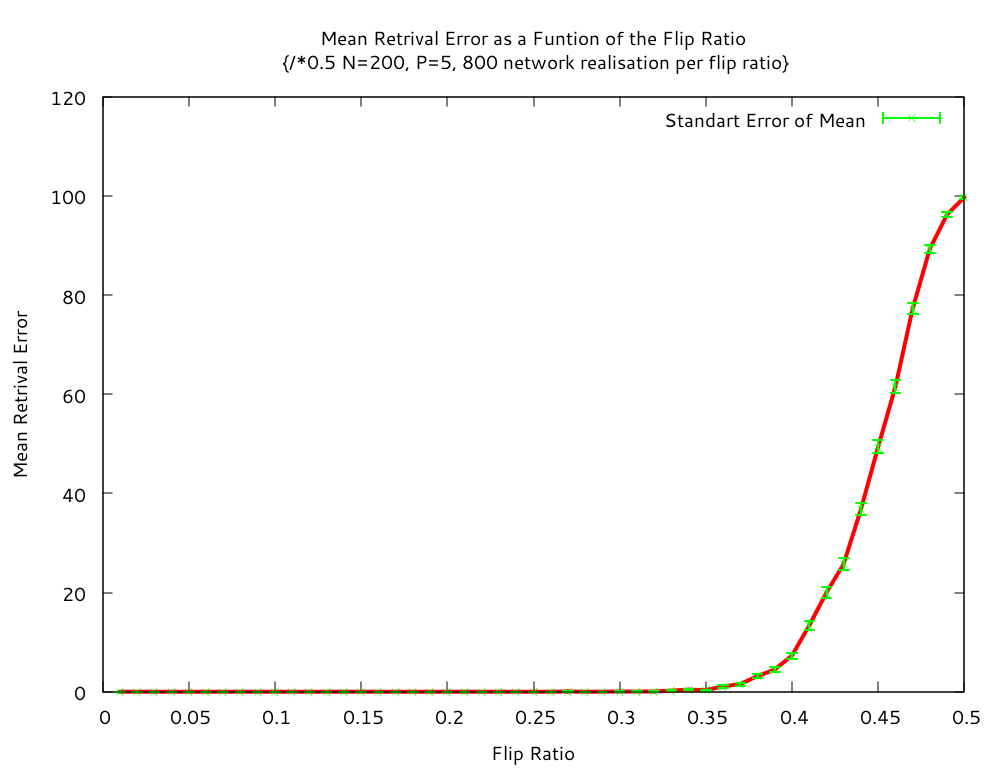
\includegraphics[scale=0.7]{img/ex11.png}
    \end{figure}
\end{center}

\subsection{Exercise 1.3 : Capacity estimation}
The number of patterns that can be stored and retrieved correctly by a neurons network depends on the number of neurons. 
In Hofield model, the storage capacity of a network is defined by :
\begin{equation}\nonumber
C_{stor} =\frac{ P^{max}}{N}
\end{equation} 
where $P^{max}$ is the maximum number of patterns that the network can retrieve correctly. \\
To study this capacity, we define the function maxLoad. We create a network of N neurons and a growing number of patterns $P$.  \\
We fix $c=0.1$. For each $P$ we try to retrieve all the patterns. When the mean error over all tries reaches $2\%$ we stop and save the number 
of patterns created as $P_{max}$. We do this $10$ times per N to have statistical average of $P_{max}$ and we deduce $\alpha_{max} = P_{max}/N$. The error on the value of $\alpha_{max}$ is the variance of $P_{max}$ divided by $N$.\\
To speed up the simulation, we start from $P = 0.1 N$ because we are sure that a network with 500 neurons, for example, will be able to
retrieve correctly at least 50 patterns. If this assumption was false, we would have known by analysing the output of the program.\\
The results are shown in table \ref{capa}.  
\begin{table}[h]\label{capa}
\begin{center}
\begin{math}
    \begin{array}{|l|c|c|c|}
    \hline
    N & 100 & 250 & 500 \\ \hline
    P_{max} & \approx 14 & \approx 38 &  \approx 77 \\ \hline
    \alpha_{max} & 0.1480 \pm  0.007423 & 0.1532 \pm  0.003322 &  0.1546 \pm  0.001550 \\ \hline
    \end{array}
\end{math}
\end{center}
\caption{Capacity storage of a network of N neurons }
\end{table}
As we could expect, we observe that the capacity of the network increases with the number of neurons. %Moreover, we see that the maximal load that we obtain corresponds extremely well to the theoretical value.\\
Note that we only retrieve one pattern at a time. If we want to retrieve a sequence of patterns, the literature says that $C_{stor}$ should not exceed 0.138\cite{prof}, otherwise, the error will propagate at each pattern of the sequence. From our table, we see that this threshold is exceeded for all N. Therefore, we should modify the model if we want to retrieve a sequence of patterns. 

\section{Exercise 2}

\subsection{Exercise 2.1 : Implementation}
Most of the functions used for the first exercise will be reused in the second. Here we want to 
implement a particular type of Hopfield Network that have a component added : the Asymmetrical 
weights. We used Oriented-Object Inheritance to derive our class hopfieldNetworkAsymmetric
from the hopfieldNetwork. Our attributes are the same than in the first part, with the addition
of :
\begin{itemize}
\item Assymweight : array of $N\times N$ that represents the projection of the weights of a 
pattern on the next one.
\item SPrev : array of $N \times t_{max}$ that contain the evaluation of $S$ for all $t \in
 [0, now]$. It is used to calculate the $\overline{S}$ that will stabilize our transitions.
\end{itemize}

We add the following methods :
\begin{description}
\item [makeAssymetricWeight] calculates the second set of weights that will be added to the standard ones according to the formula : 
$w_{ij}^L = \frac{\lambda}{N}\sum_{\mu=1}^P \xi_i^{\mu+1} \xi_j^{\mu}$
\item [filterfunction] The implementation of our filter function. We chose the Heaviside function : $G(t) = \frac{1}{\tau} \Theta (-t + \tau)$
\item[dynamic] It is a two step function that updates the state of the network at each time-step. Since we do synchronous update, all the variables are vectors.
\begin{enumerate}
    \item Calculate the new  $\overline{S}$ from the memory of all previous states, as $\overline{S} = \sum_{t'=0}^{t} G(t')S(t-t')$
    \item Update the state of all the neurons in one step, 
according to the formula : $S_i = \textrm{sign}\big(\sum_{j=1}^N w_{ij}S_j + w_{ij}^L\overline{S} \big)$ using the two weights matrix with the current and filtered state of the network
\end{enumerate}  
\end{description}


\begin{figure}\label{seq}
    \begin{center}
    \caption{Illustration of the sequential behaviour}
    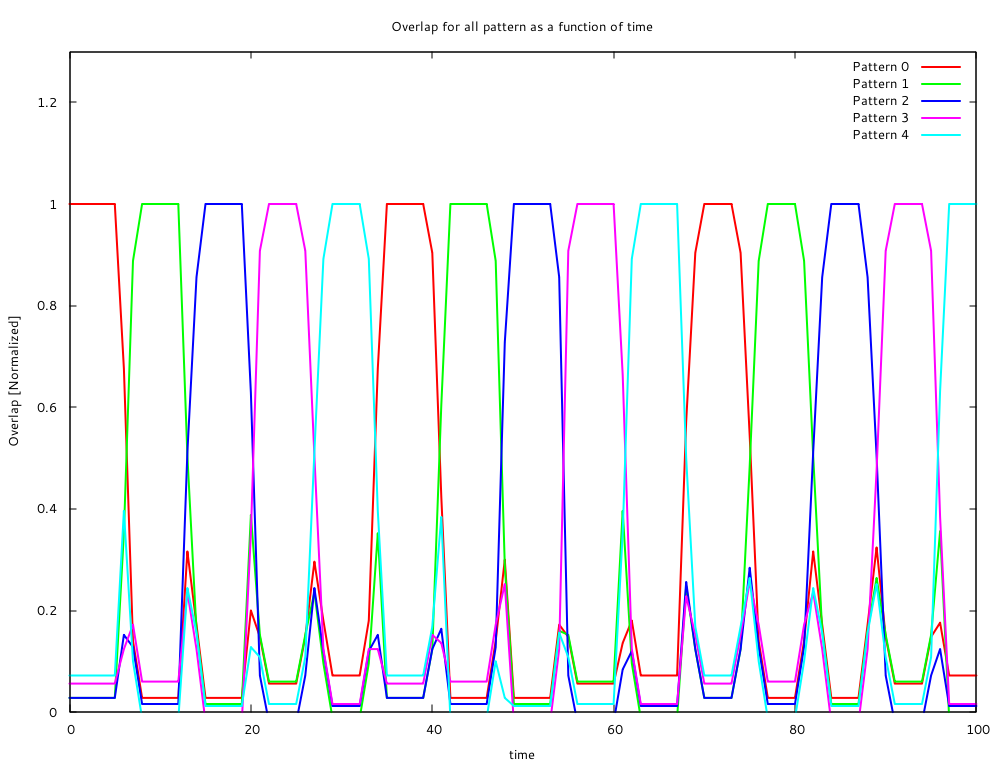
\includegraphics[scale=0.3]{img/ex21.png}
    \end{center}
\end{figure}
The process is the same as in exercise 1. If we plot the overlap for all the patterns at every
time step, we see that our network goes from one stored pattern to another (Figure~\ref{seq})


\subsection{Exercise 2.2 : $\lambda$ range estimation}
We consider that we have a {\it sequential behaviour} when all patterns $\mu$ are "visited", meaning that the overlap $m^{\mu}$ reaches the value 1 $\forall \mu$.\\ 
Keeping N=500,P=10 and $\tau$=8 fixed, we simulate the network with different values of $\lambda$. The minimum value for which we can observe this behaviour is 
\begin{center}
$\lambda_{min} \approx 0.9$
\end{center}
For values below this one, the network gets stuck in a particular pattern. This is in accordance with the new weights formula. When $\lambda$ is very low, the additional term becomes negligible and we are back to the previous model, where we converged to one specific pattern. \\ 
For high values of $\lambda$, we observe that the network skips some patterns, meaning that the overlap $m^{\mu}$ increases but does not reach 1. Here the influence from the previous pattern is too strong, and the model becomes unstable. We found :
\begin{center}
$\lambda_{max} \approx 3.6$
\end{center}
Due to the random generation of some variables, the values of $\lambda_{min}$ and $\lambda_{max}$ are approximative.
\subsection{Exercise 2.3 : Estimation of the transition time}
The transition time (that we defined as the time the network stays in a given frame with a overlap of 1) depends on the filter function parameter $\tau$, and on $\lambda$.

We run our network 5 times for each configuration ($\lambda \in [1.3, 1.7, 2.2, 2.5]$ and 
$\tau \in [1, 25]$), saving the transition time on a file to plot it with gnuplot. 

The results
are displayed in Figure~\ref{transtime}. If we discard the small values of $\tau < 5$, we
see a linear behaviour, the transition time increasing with $\tau$. This is what we wanted to obtain in this model, e.g., slowing down the transition time. Increasing $\lambda$ shifts the curve downward. This behaviour is in accordance with what we observed in the previous section.  
The slope of the curve is fixed by other parameters.
\begin{figure}\label{transtime}
    \begin{center}
    \caption{Mean retrieval error as a function of the flip ration $c\in[0.01, 0.51]$.  }
    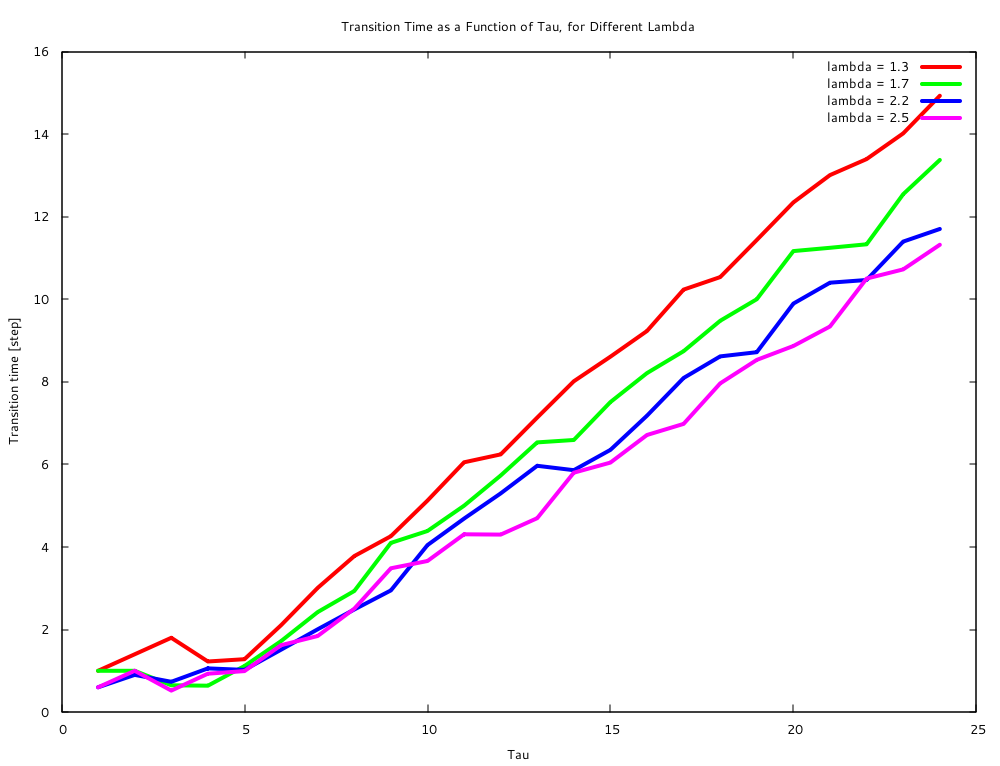
\includegraphics[scale=0.5]{img/ex23.png}
    \end{center}
\end{figure}


\subsection{Exercise 2.4 : Sequence Storage Capacity}

By varying $P$ with $N$ fixed, we saw that increasing the number of patterns stored leads the network
to never achieve an overlap of 1, or only for a few patterns. For example with $N = 500$ and $P = 40$ only one pattern, the $4^{th}$, was retrieved correctly. If we print the overlap we see that for a high $P$, the mean overlap is considerably low. \\
We fixed all the parameters of our network, except the number of patterns $P$ and the size of the
network $N$. For every N we increased $P$ until one of the pattern stored was skipped during an iteration. The results are displayed on Table~\ref{capaseq}. Again due to the randomness of the process
we show here statistical average, on a small number of trials. 

\begin{table}[h]\label{capaseq}
\begin{center}
\begin{math}
    \begin{array}{|l|c|c|c|}
    \hline
    N & 250 & 500 & 1000 \\ \hline
    P_{max} & 15 & 33 & 52 \\ \hline
    \alpha_{max}& 0.06 & 0.066 & 0.052\\ \hline
    \end{array}
\end{math}
\end{center}
\caption{Sequence storage capacity  of a network of N neurons}
\end{table}
Comparing these results to the ones obtained with a non-sequential network model, we observe that the maximum load is significantly lower (divided by a factor $\approx 2.66$). However the threshold value of  $C_{stor}$ = 0.138 is never exceeded. Therefore, this model allows the network to retrieve a sequence of patterns, but it reduces its storage capacity. 


\begin{thebibliography}{}
\bibitem{prof} W. Gerstner, W. Kistler, R. Naud, L. Paninski, \textit{Neuronal Dynamics : from single neurons to networks and models of cognition}, Cambridge University Press, 2014.
\end{thebibliography}
\end{document}